\documentclass[11pt]{article}

\usepackage[margin=0.76in]{geometry}
\usepackage{indentfirst}
\usepackage{graphicx}
\usepackage{float}
\usepackage{wrapfig}
\usepackage{lipsum}
\bibliographystyle{siam}

\title{The Neural Basis of Loss Aversion in Decision-Making Under Risk}
\author{
  Chang, Siyao \\
  \texttt{changsiyao}
  \and
  Gong, Boying\\
  \texttt{boyinggong}
  \and
  Hsieh, Benjamin\\
  \texttt{BenjaminHsieh}
  \and
  Qiu, Brian\\
  \texttt{brianqiu}
  \and
  Zhu, Jiang\\
  \texttt{pigriver123}
}



\begin{document}
\maketitle

\par Our paper is the \textit{Neural Basis of Loss Aversion in 
Decision-Making Under Risk} \cite{Tom2007LossAversion}.
The experiment investigates the
phenomenon of loss aversion - where individuals' decisions are influenced by 
the amount of potential loss more than they are by the amount of potential 
gains. 

\par 
Our analysis of the paper aims to verify this result and to replicate the 
connections found between neural loss aversion (shown in brain activation) and 
behavioral loss aversion (shown in the actual decisions to accept or reject 
gambles based on potential gain/loss). Our work has found that the neural loss 
aversion is significantly correlated with behavioral loss aversion in specific 
regions of the brain. Our work also shows that there are increasing neural 
activation to increasing potential gains and negative neural activation to 
increasing potential loss.

\section{Introduction}
The experiment conducted in the paper itself involved giving 16 subjects a 
total of 256 combinations of gain/loss in dollars with a 50 percent chance of 
winning. The subject's decision of whether to accept or reject each proposed 
gamble was recorded as well as the their brain activity in the fMRI machine as 
they made their decision. The neural activity is measured in BOLD signals.

\par 
We determine the beta coefficients for each voxel in the subject's brain based 
on a linear regression on the BOLD signal data. We use these coefficients as 
evidence for increasing activation in certain voxels in the brain when the 
subject is making a decision to accept or reject, and so in this way we have a 
proxy for which regions of the brain are involved with loss-aversion 
decision-making. We also determine the p-values to validate these results.

\par 
We also run a logistic regression to determine each subject's willingness to 
accept or reject based on the values of potential loss and gain. This is the 
measure of behavioral loss aversion, and in the end we correlate this with our 
neural loss aversion, making it clear that increasing gains correspond to 
increasing activity in certain parts of the brain.  

\section{Data}
\subsection{Overview}
The study used 16 right-handed, healthy, English-speaking participants 
recruited through ads posted on UCLA. Out of 16 subjects, 9 were female and 
the mean age was 22 $ \pm $ 2.9 years.\cite{Tom2007LossAversion} 

\subsection{Behavioral Data}
The behavioral data consists of each subject undergoing 3 trial runs for the 
``gamble'' task, in which each subject is presented with a combination of 
potential monetary gains and losses given a 50/50 chance of to win/loss. Each 
trial run consists of 86 different combinations of rewards/penalties spread 
out across 474 seconds. Intervals between each onset of task range from 4 to 
8 seconds. Subjects were given the 4 choices in response to each gambling 
proposal:
\begin{enumerate}
  \item Strong Accept
  \item Weak Accept
  \item Weak Reject
  \item Strong Reject
\end{enumerate}
The choices are recorded by denoting response numbers 1, 2, 3, and 4, 
respectively. Furthermore, the response time for each gambling decision was 
recorded in seconds. 
\subsection{BOLD Data}
\subsubsection{RAW Data}
Raw Blood-oxygen-level dependent (BOLD) imaging data were collected from each
subject as he/she performed the gamble tasks. 240 time scans were done on each
run with a time between each scan of 2 seconds. So total scanning time is 480
seconds. Each scan consists of a snapshot consisting of a 64 by 64 by 34 image
matrix.
\subsubsection{Standardized Data}
We also used the provided filtered, preprocessed BOLD data. Again, 240 time 
scans were done on each run with a time between each scan of 2 seconds. So 
total scanning time is 480 seconds. Each scan consists of a 91 x 109 x 91 
snapshot image matrix. Besides the preprocessing, this data also has the 
advantage of each voxel being mapped to a standard MNI template. There are 
also 4 model conditions, with events corresponding to 
\begin{enumerate}
  \item Task
  \item Parametric Gain
  \item Parametric Loss
  \item Distance from Indifference
\end{enumerate}
We refer to this provided dataet as filtered or standardized to differentiate 
from the raw
BOLD dataet of which we preprocess and also run analyses on.

\subsection{Processing}
Before we run our analyses and fit betas to our data, we first take a few 
steps to clean the raw BOLD dataets. We graph the dvars (RMS of the signal 
derivatives) and the framewise displacement, and we use that in conjunction 
with the mean signal of the BOLD data to determine outliers to remove. The 
BOLD data is smoothed spatially in order to make clearer the signal in 
relation to the noise present. We also take the mean signal of the BOLD data 
across the run and plot the histogram for each run and subject to help 
manually determine a good threshold for a mask we use to isolate more active 
voxels in the brain. This helps us find beta coefficients for more relevant 
voxels. We also model and remove the linear and quadratic drift that may be 
present in the runs. We use subject 2 run 2 to show an example of our outliers r
esults. (Green dotted line in DVARS: thredhold for outliers, Greenline in mean 
signal: fitted smooth curve of the bold signal)

\begin{figure}[H]
    \centering
        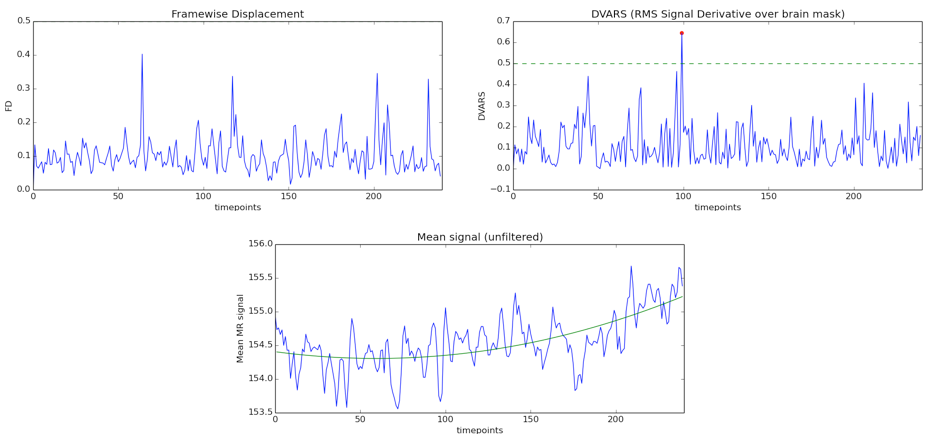
\includegraphics[scale=0.55]{figures/processing.png}
    \caption{DVARS, Framewise Displacement and Data mean for subject 2 run 2}
\end{figure}

\section{Models and methods}

\subsection{Models}

In this section, we present the models we used to find the relationship between 
behavioral and neural loss aversions cross participants as well as how 
participants react to different loss and gain levels. For behavioral data, we 
fit the logistic regression models for each subject and use the coefficients of 
loss and gain to calculate the behavioral loss aversion levels. For neural d
ata, we fit both linear multiple regression models and mixed-effects models in 
order to collapse three runs for each subject into one model. We analyze the 
fMRI data using both models and compare the results we obtained. Neural loss 
aversion levels are calculated using the coefficients of loss and gain, and 
are done for both the raw and filtered dataets. However we do not run a mixed 
effects model on the filtered dataet due to size constraints.   

\subsubsection{Behavioral analysis using Logistic regression}

We fit a Logistic regression model on the behavioral data to examine how the 
response of individuals relates to the size of potential gain and loss of a 
gamble. Originally there are four acceptability judgments categories, here we 
collapse the categories into binary response (accept/reject). 
Following is the model:

\begin{equation}
\textrm{log}\frac{p(X)}{1-p(X)} = \beta_0 + \beta_{loss} *X_{loss} + 
\beta_{gain} * X_{gain}
\end{equation}

where $X_{loss}$ and $X_{gain}$ are the potential loss and gain value 
separately, $Y_{resp}$ is a categorical independent variable representing the 
subjects' decision on whether to accept or reject the gambles:

\begin{displaymath}
Y_{resp} = \left \{ \begin{array}{ll}
1 & \textrm{If the subject accepted the gamble.} \\
0 & \textrm{If the subject rejected the gamble.}
\end{array} \right .
\end{displaymath}

Then we calculate the behavioral loss aversion ($ \lambda $) for each subject 
as follows, note that for simplicity, we collapse 3 runs into one model for 
each participant.

\begin{equation}
\lambda = -\beta_{loss} / \beta_{gain}
\end{equation}

We use $\lambda$ as the metric for the degree of behavioral loss aversion for 
each participant. 

\subsubsection{Linear Regression on fMRI data}

\textbf{Raw Data Regression}

For each voxel $i$, we fit a multiple linear model:

\begin{equation}
Y_{i} = \beta_{i, 0} + \beta_{i, gain} * X_{gain}  + \beta_{i, loss} *X_{loss} 
+ \beta_{i,ldrift} *X_{ldrift} + \beta_{i, qdrift} * X_{qdrift} 
+ \epsilon_i
\end{equation}

where $Y_{i}$ is the BOLD data of voxel $i$,  $X_{ldrift}$ and $X_{qdrift}$ are 
linear and quadratic drift terms. \\

\textbf{Pre-processed Data Regression}

For each voxel $i$, we fit a multiple linear model:

\begin{equation}
Y_{i} = \beta_{i, 0} + \beta_{i, gain} * X_{gain}  +  \beta_{i, loss} *X_{loss} 
+ \epsilon_i
\end{equation}

where $Y_{i}$ is the BOLD data of voxel $i$.
For the pre-processed data, we no longer need to include the drift terms. The 
drifts are taken care of in the pre-process steps.

For each voxel, we calculate the 
neural loss aversion $\eta_i$:

\begin{equation}
\eta_i = (-\beta_{loss}) - \beta_{gain}
\end{equation}

Using the voxelwise neural loss aversion, we do a region-specific analysis on 
BOLD data for each participant. That is, we calculate and plot heat maps of the 
t valuesfor $\beta_{loss}$ and $\beta_{gain}$ for each participant to find out 
the regions with significant activation and regions, which show a significant 
positive or negative correlation with increasing loss or gain levels.

\subsubsection{Mixed-effects model on fMRI data}

The fact that we have 3 runs of data for each participants leads us to consider 
using mixed effects model to analysis the data set. The mixed effect model adds 
a random effects term, which is associated with individual experimental units 
drawn at random from a population. In this case, it measures the difference 
between the average brain activation in run i and the 
average brain activation in all three runs. For each voxel $i$, we fit the 
following mixed-effects models, note that here we only include the intercept 
term for random effects (the following model is for the raw data, for the 
filtered data, we subtract the drift terms).

\begin{equation}
Y_{i, k} = \beta_{i, 0} + \beta_{i,1} *X_{ldrift} + \beta_{i, 2} * X_{qdrift} 
+  \beta_{i, loss} *X_{loss} + \beta_{i, gain} * X_{gain}  + \gamma _{i, k} 
+ \epsilon_{i, k}, \quad k =1, 2, 3
\end{equation}

Then we calculate the neural loss aversion level and plot heat maps in the same 
way as the about section for multiple linear regressions and compare the 
results of two models. 

\subsubsection{Whole brain analysis of correlation between 
neural activity and behavioral response across participants}

We then apply the above model on the standard brain to analysis the neural 
activity and behavioral response across participants. For each participant, 
we pick up several regions with highest activation level, calculate the mean 
neural loss aversion $\bar{\eta}$ within these specific region. Thus we could 
examine the relationship between neural activity and behavioral using the 
following regression model:

\begin{equation}
\lambda = \alpha_0 + \alpha_1 * \eta + \epsilon
\end{equation}

where the sample size is the number of participants(16). 

\subsection{Methods}

\subsubsection{Cross-validation}

To estimate how accurately a predictive model will, we do a k-fold 
cross-validation for each linearmodel. We choose to use 10 fold 
cross-validation for both behavioral and neural model,
which means the original sample is randomly partitioned into 10 equal sized 
subsamples. 
\par
In the behavioral analysis using Logistic regression, since the response 
variables are binary, we calculate the misclassification error rate to 
summarize the fit. In the neural linear regression model using BOLD data, we 
use the mean squared error to summarize the errors.

\subsubsection{ROC curve}

ROC curve and AUC are mostly used for model selection of a binary classifier. 
In the behavioral analysis, we use logistic regression as the binary 
classifier for the response of reject and accept. To check the performance of 
the logistic classifier as its discrimination varied, we plot the ROC 
(receiver operating characteristic) curve and calculate the corresponding AUC 
(areas under the curve). In the model analysis, we prefer models with bigger 
AUC values.

\subsubsection{Inferences on regression models}

After fitting regression models on our BOLD and behavioral data, we assess 
and validate our models. We calculate the following statistics:
\begin{itemize}
\item \emph{t-statistics and p-value} Calculate the t-statistics and p-value for 
our beta coefficients to check whether our beta parameters are statistically 
significant.
\item \emph{R-Squared value and the adjusted R-squared value} Calculate 
R-Squared value and the adjusted R-squared value to see how close the data are 
to the fitted regression line, that is the proportion of variability of the 
response data explained by the model.
\end{itemize}

\subsubsection{Normality assumption on linear models}

Since the performance of the test statistic of linear models are largely 
depend on the normality assumption on the independent variables, the check of 
normality assumption is indispensable. We choose the following methods for 
normality assumption:

\begin{itemize}
\item{QQ plot} The quantile-quantile plot (QQ plot) is the most commonly used 
visualization method to check the validity of a distribution assumption. The 
basic idea is to compute the empirical quantile the and compare it with the 
theoretically expected value of a normal distribution. If the data follow a 
normal distribution, then the points on the Q-Q plot would fall on a straight 
line. 
\item{Residuals vs. fits plot} A residuals vs. fits plot is another most 
frequently created plot. Under the normality assumption, the residuals should 
be independent and scatted around.
\end{itemize}

\subsubsection{ANOVA test}

In our dataet, each participant repeated the test for three times, in other 
words there are data of 3 runs for each subject. Before collapsing the three 
runs into one model, we need to check the assumption whether they are i
ndiscriminate.  To do this, we perform an ANOVA test on each subject to check 
the difference of means across runs. The significance of an AVOVA test may 
show that there are difference across runs, thus we may seek other methods to 
eliminate the influence due to the variance across runs.

\subsubsection{Multiple Test correction}

In statistical inference for fMRI data, usually we have more than tens of 
thousands of hypothesis tests, thus massive multiple correction problems. 
Using thresholds without correction could be problematic. Common multiple 
correction methods (such as Bonferroni) require adjusting the p-values. 
However, imposing high statistical thresholds that may mask voxels that do have 
real effects. To avoid this loss, we use uncorrected threshold and choose the 
threshold on a case-by-case basis.


\subsubsection{Cluster analysis}

We use K-means clustering to detect the homogeneity of regions. We concatenate 
the betas obtained from linear models and the coordinate of voxels as the 
clustering vector (dimension = 16 + 3 = 19). Then do cluster analysis for beta 
gains and beta loss separately to detect regions activated by increasing beta 
losses and beta gains.


\section{Results}

\subsection{Behavioral analysis}

We performed statistical analysis using both Python and R (The original paper 
use R package to fit the Logistic models). We use the library 
\emph{scikit-learn} in Python and the \emph{glm} function in \emph{stats} in R 
to fit the models. Models from two library yields the same results. We shows 
the plot of the behavioral loss aversion $\lambda$ for every subject 
(median=1.94, mean=2.18, min=0.99, max=0.75). This result is consistent with 
that of the paper, which indicate that participants are indifferent to gambles 
whose gain are approximately twice as the loss. 


\begin{wrapfigure}{r}{0.55\textwidth}
  \begin{center}
    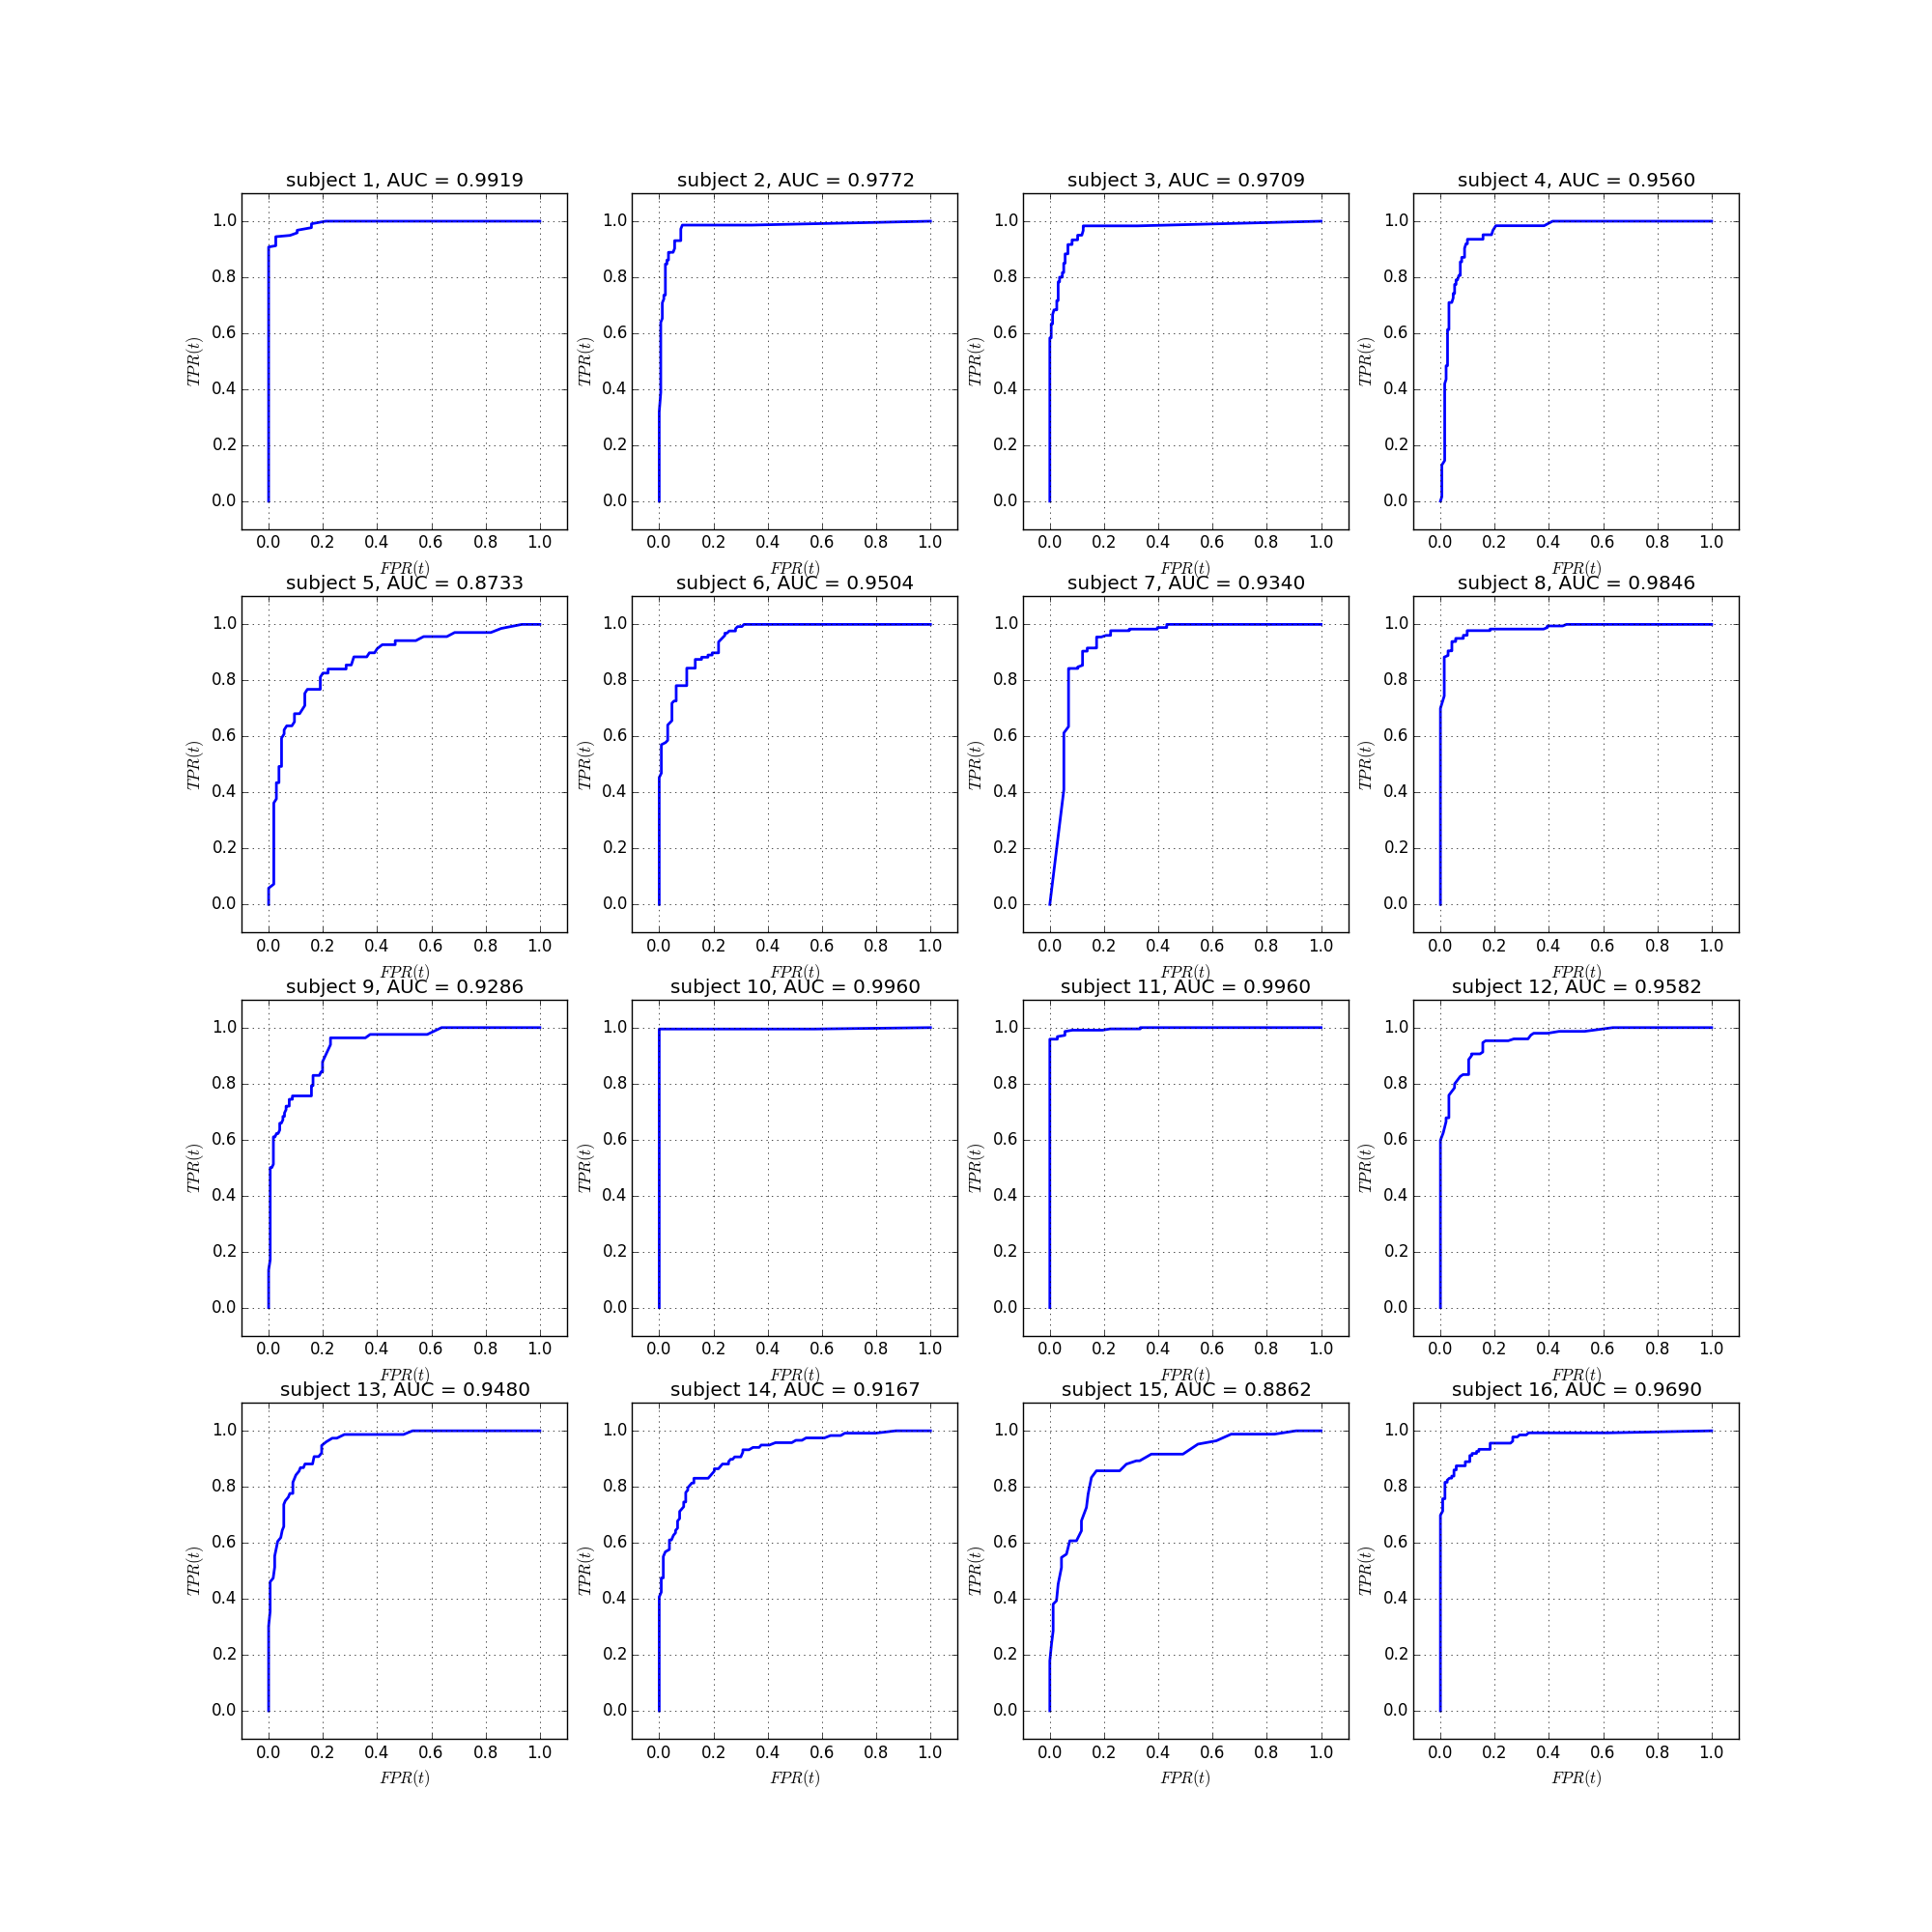
\includegraphics[width=0.53\textwidth]{figures/Regression1/roc_curve.png} 
    \caption{ROC Curve for all subjects}
  \end{center}
\end{wrapfigure}

Following are the model diagnosis:

\begin{itemize}
\item \emph{Accuracy on the training dataet} We uses the fitted models on the 
original dataets and compared the estimated class and the true class using the 
Logistic classifier. The accuracy (proportion of correct classifies) of 
Logistic models (for 16 participants, 16 
models in total) on the training set yielded a median of 89.78\% (min=80.97\%, 
max=99.21\%).
\item \emph{Cross-validation} We did the model evaluation using 10-fold 
cross-validation for every subject, they are still performing accuracies of a 
median of 89.86\% (min=79.92\%, max=98.45\%).
\item \emph{ROC Curve and AUC} We plot the ROC (receiver operating 
characteristic) curve to see how the logistic classifier perform as the its 
discrimination threshold is varied for every subject. We also calculated the 
corresponding AUC (areas under the curve) for every curve, the area is large 
for the models (min=0.886, max=0.996), which shows the model performs well 
under various discrimination threshold.

\end{itemize}

\begin{figure}[H]
    \centering
        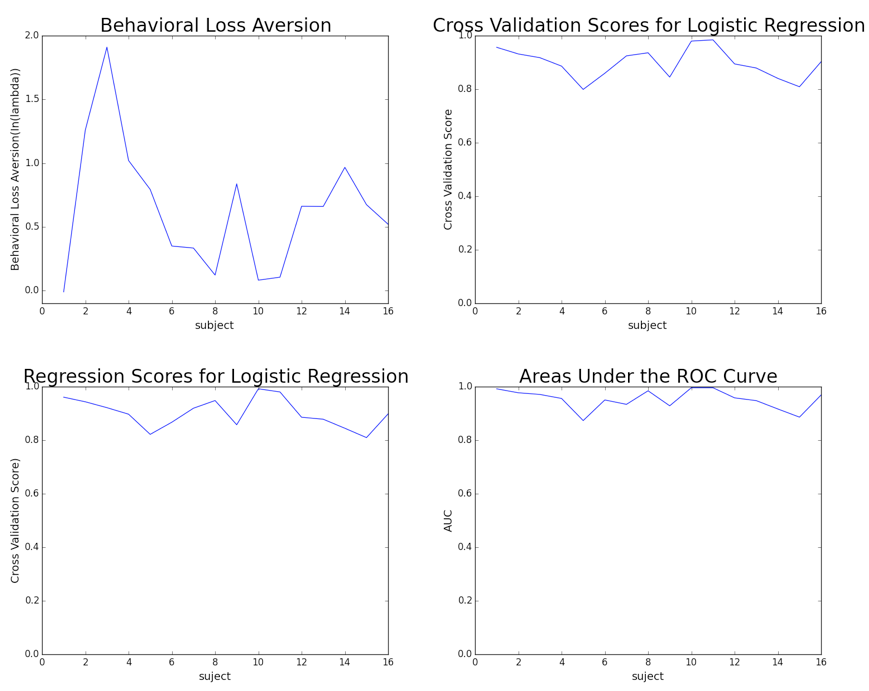
\includegraphics[scale=0.4]{figures/Regression1/logistic_summary.png}
    \caption{Results summary of the Logistic regression}
\end{figure}

\subsection{Linear Regression on BOLD data}

The topic we are interested in exploring is whether loss aversion reflects 
the engagement of distinct emotional processes when potential gains and 
losses are considered. In the process, we want to explore the correlation 
between neural and behavioral loss aversion in whole brain analysis. We also 
want to try to identify the regions of brain that is more activated by this 
loss aversion activity.

Since we want to explore the correlation between neural and behavioral loss 
aversion, the second step is to find out the neural loss aversion. In order 
to find the neural loss aversion, we perform a linear regression on the BOLD 
data against the parametric gain values and the parametric loss values, as 
explained in our model section. (While implementing the linear regression for 
the raw data, we also added linear and quadratic drift in our model. These 
drift terms are modeling for gradual drifts across the time series.)

We are especially interested in the beta coefficients of our parametric gain 
and parametric loss regressors, which are the first two columns in our design 
matrix. To find out the regions with significant positive or negative 
correlation with increasing gain or loss levels, we calculate the t statistics 
for each voxel. Plotting heat maps of the t statistics will show us regions 
with significant parametric increase in fMRI signal to increasing potential 
gains and regions with significant parametric decrease to increasing potential 
losses.

By looking at the heatmaps, we can get a general idea of how potential gains 
and potential losses affect brain activation. We can also identify the areas 
that have large coefficients; these are the areas that the brain activation is 
highly connected to the potential gains and losses. We choose the preprocessed 
data for subject 2 to plot heat maps since the preprocessed data is mapped 
onto the standard brain. We plot slices 31 to 60 from the third dimension of 
the brain (top to bottom). The red color is associated with positive t values 
and blue color is associated with negative t values. We can see that for the 
significant t values for the gain coefficients are mostly positive while the
the significant t values for the loss coefficients are mostly negative.

\begin{figure}[H]
    \centering
      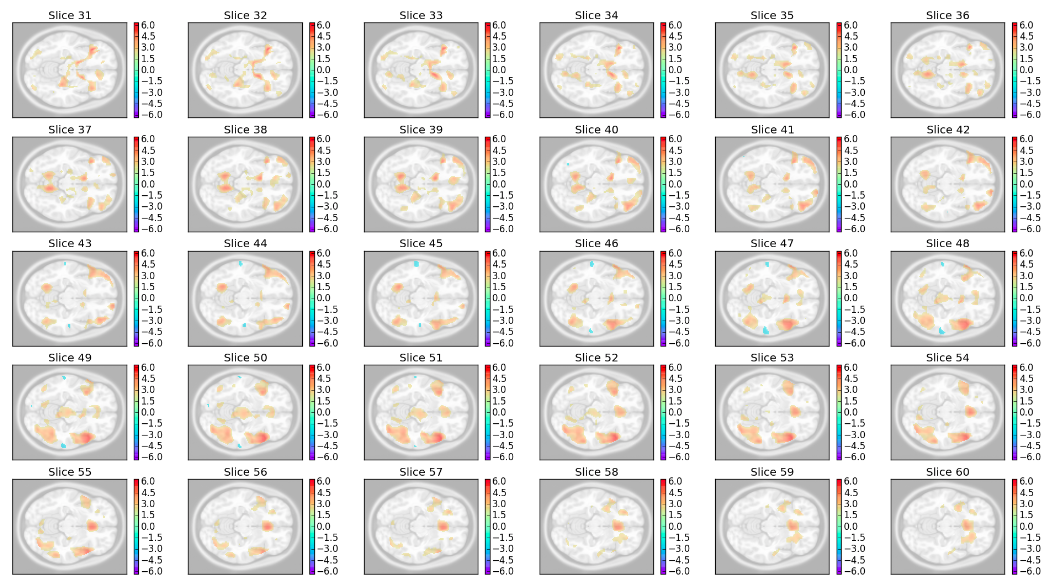
\includegraphics[scale=0.4]{figures/Regression2/t_gain_standard_sub2.png}
    \caption{t values of the gain coefficients for subject 2}
\end{figure}

\begin{figure}[H]
    \centering
      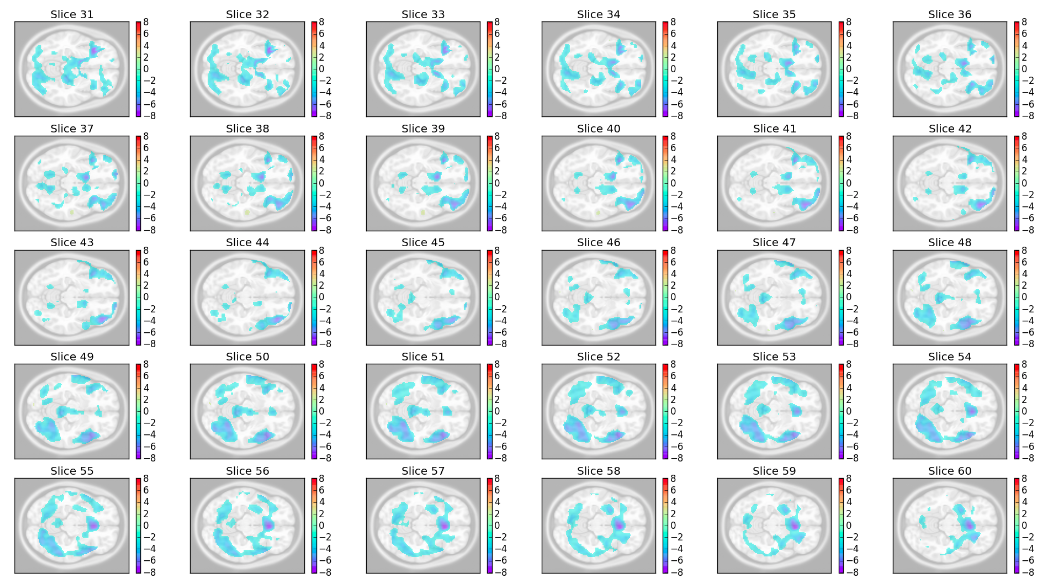
\includegraphics[scale=0.4]{figures/Regression2/t_loss_standard_sub2.png}
    \caption{t values of the loss coefficients for subject 2}
\end{figure}

We can see that significant areas for the gain coefficients and those of the 
loss coefficients are mostly the same. This suggests that opposite of what 
most people believes that increasing potential losses should affect the areas 
of the brain that mediate negative emotions in decision-making, potential 
losses were represented by decreasing activity in the same areas that are 
sensitive to potential gains.

From the gain and loss coefficients, we can also compute the neural loss
aversion. This serves the next step of looking at the correlation between
neural and behavioral loss aversion. The neural gain and loss coefficients
were broadly distributed and spanned zero, so it is not possible to compute
the ratio of loss to gain coefficients, nor does it make much sense.
Therefore, we compute the neural loss aversion at every voxel by subtracting
the slope of the gain response from the (negative) slope of the loss response.
With the neural loss aversion values calculated, we can explore how loss
aversion affects brain activation when potential gains and losses are
considered.

\subsubsection{Model Diagnosis for linear regression}

From the results of the QQ plot, we can see that in this randomly picture. The 
residuals are approximately normal distribution and showed constant variance. 
The green line is the QQ plot 
of the normal distribution. The blue line is the QQ plot of residuals. They 
look quite similar. The second plot is the scatter plot of the residuals. We 
can see that the residuals are approximately equally distributed by 0. This 
means that the residuals are not correlated to the fitted values. To conclude, 
the residuals are approximately normal distributed.

\begin{figure}[H]
    \centering
        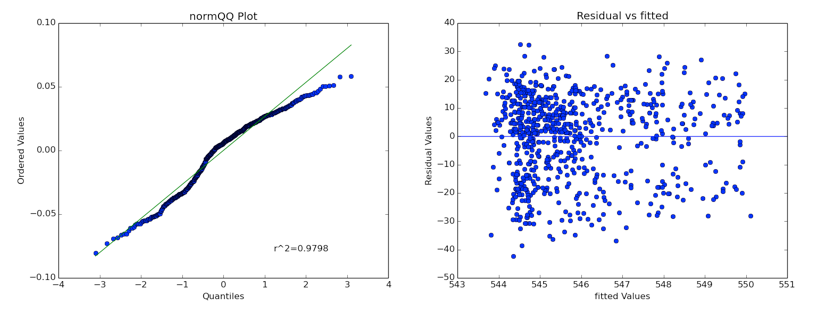
\includegraphics[scale=0.4]{figures/Regression2/diagnosis.png}
    \caption{QQ plot and fitted-residual plot for a randomly chosen voxel}
\end{figure}

\subsubsection{Cluster Analysis for betas from linear regression}

We applied k-means clustering and minibatch k-means clustering on the betas 
obtained from the neural linear regression models. We choose 20 as our number 
of clusters. Following are the slices of our clustering results. We will use 
the clustering maps to detect underlying significant regions in the later part 
in the whole brain analysis.

\begin{figure}[H]
    \centering
        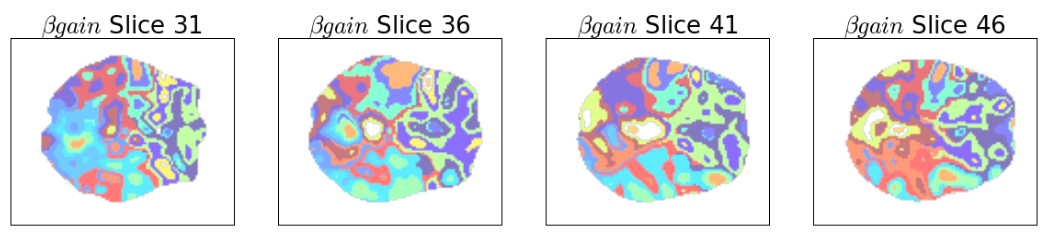
\includegraphics[scale=0.4]{figures/Regression2/beta_gain_cluster.png}
    \caption{Clusters for beta gains in linear regression across 
    subjects (\#clusters = 20)}
\end{figure}

\begin{figure}[H]
    \centering
      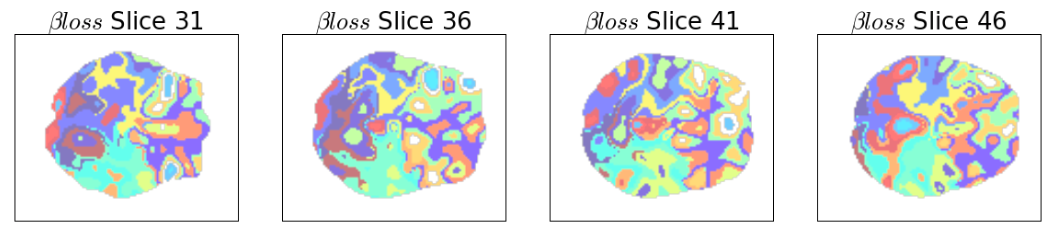
\includegraphics[scale=0.4]{figures/Regression2/beta_loss_cluster.png}
    \caption{Clusters for beta losses in linear regression across subjects 
    (\#clusters = 20)}
\end{figure}


\subsection{Mixed-effects model on fMRI data}
First, we did the ANOVA test for each subject each voxels, grouping by runs. 
The high proportion of significant ANOVA F-test (after Bonferroni correction 
under 0.05 significant level) shows that mixed effects model may perform well 
when collapsing three runs into one model. 
\begin{figure}[H]
    \centering
        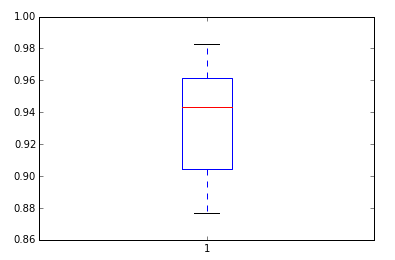
\includegraphics[scale=0.45]{figures/anova_prop.png}
\caption{Box plot of the significant ANOVA test}
\end{figure}
The mixed-effects model for each subject yielded a a median of 9.4\% (min=6.4\%, 
max=21.5\%) and 8.3\% (min=4.6\%, max=15.4\%) of proportion of significant 
coefficient for gain and loss separately. 

The run time issue (takes 26 hours for raw data on a 1.3GHz Intel Core i5 
Macintosh Machine) makes it rather hard to fit the standard brain data (the 
size is 7 times of the raw data) to a mixed-effects model on our computer. 
We performed the mixed-effects model on the raw data only. Due to the limited 
space, we did not presented the heat map in the paper. Figures are under the 
figure folder.

\newpage

\subsection{Whole brain analysis of correlation between neural activity and 
behavioral response across participants}

\begin{wrapfigure}{r}{0.65\textwidth}
  \begin{center}
    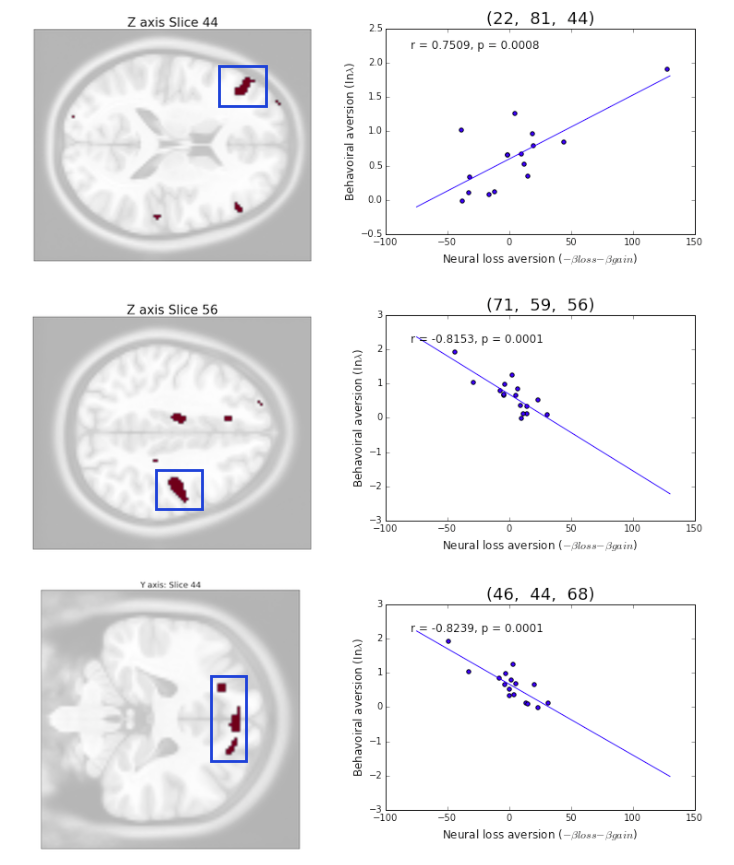
\includegraphics[width=0.63\textwidth]{figures/Regression3/corr_neu_bah.png} 
  \end{center}
\end{wrapfigure}

The figure on the right shows the correspondence between neural and behavioral 
loss aversion. Left panel presents statistical maps of the correlation between 
neural and behavioral loss aversion in whole brain analysis (Significant level 
= 0.001). We pick 2 slices by Z axis, one slice by Y axis and analyzed 3 
regions. Right panel presents scatterplots of behavioral versus neural loss 
aversion in corresponding clusters. Regression lines and p-values were computed 
using multiple linear regression. While in the original paper there is no 
clusters which shows negative significant correlation between the neural loss 
aversion and behavioral loss aversion, our results shows that there are both 
significant positive correlation and significant negative correlation. We use 
the following three clusters to illustrate these.

\begin{itemize}
\item \emph{Region 1: Voxel coordinates [22, 81, 44]} The corresponding 
millimeters coordinates is [46, 36, 16], which is very closed to L 
inferior/middle frontal (-48.5, 24.7, 17.0). In this cluster, the number of 
voxels significant is 95, the range of x, y and z is (19, 25), (79, 86), 
(41, 50) separately.
\end{itemize}

\begin{itemize}
\item \emph{Region 2: Voxel coordinates: [71, 59, 56]} In this cluster, the 
number of voxels significant is 151, the mean p-value is 0.000240. For the 
region, the range of x, y and z is (63, 71), (54, 60), (52, 57) separately. 
This cluster showed significant negative correlation between behavioral loss 
aversion and neural loss aversion.
\item \emph{Region 3: Voxel coordinates: [46, 44, 68]} In this cluster, the 
number of voxels significant is 136, the mean p-value is 0.000522. For the 
region, the range of x, y and z is (33, 57), (40, 45), (61, 69) separately. 
This cluster also showed significant negative correlation between behavioral 
loss aversion and neural loss aversion.

\end{itemize}

\newpage

\emph{Figure S1} Regions with significant correlation between the parametric r
esponse to potential loss and behavioral loss aversion (ln($\lambda$)) across 
participants (Significant level = 0.001).  Most of the regions show significant 
negative correlation, only one region showed significant positive correlation. 
This is slightly different from the original paper, in which no regions showed 
significant positive correlation, which is consistent with the original paper
\cite{Tom2007LossAversion}.

\begin{figure}[H]
    \centering
        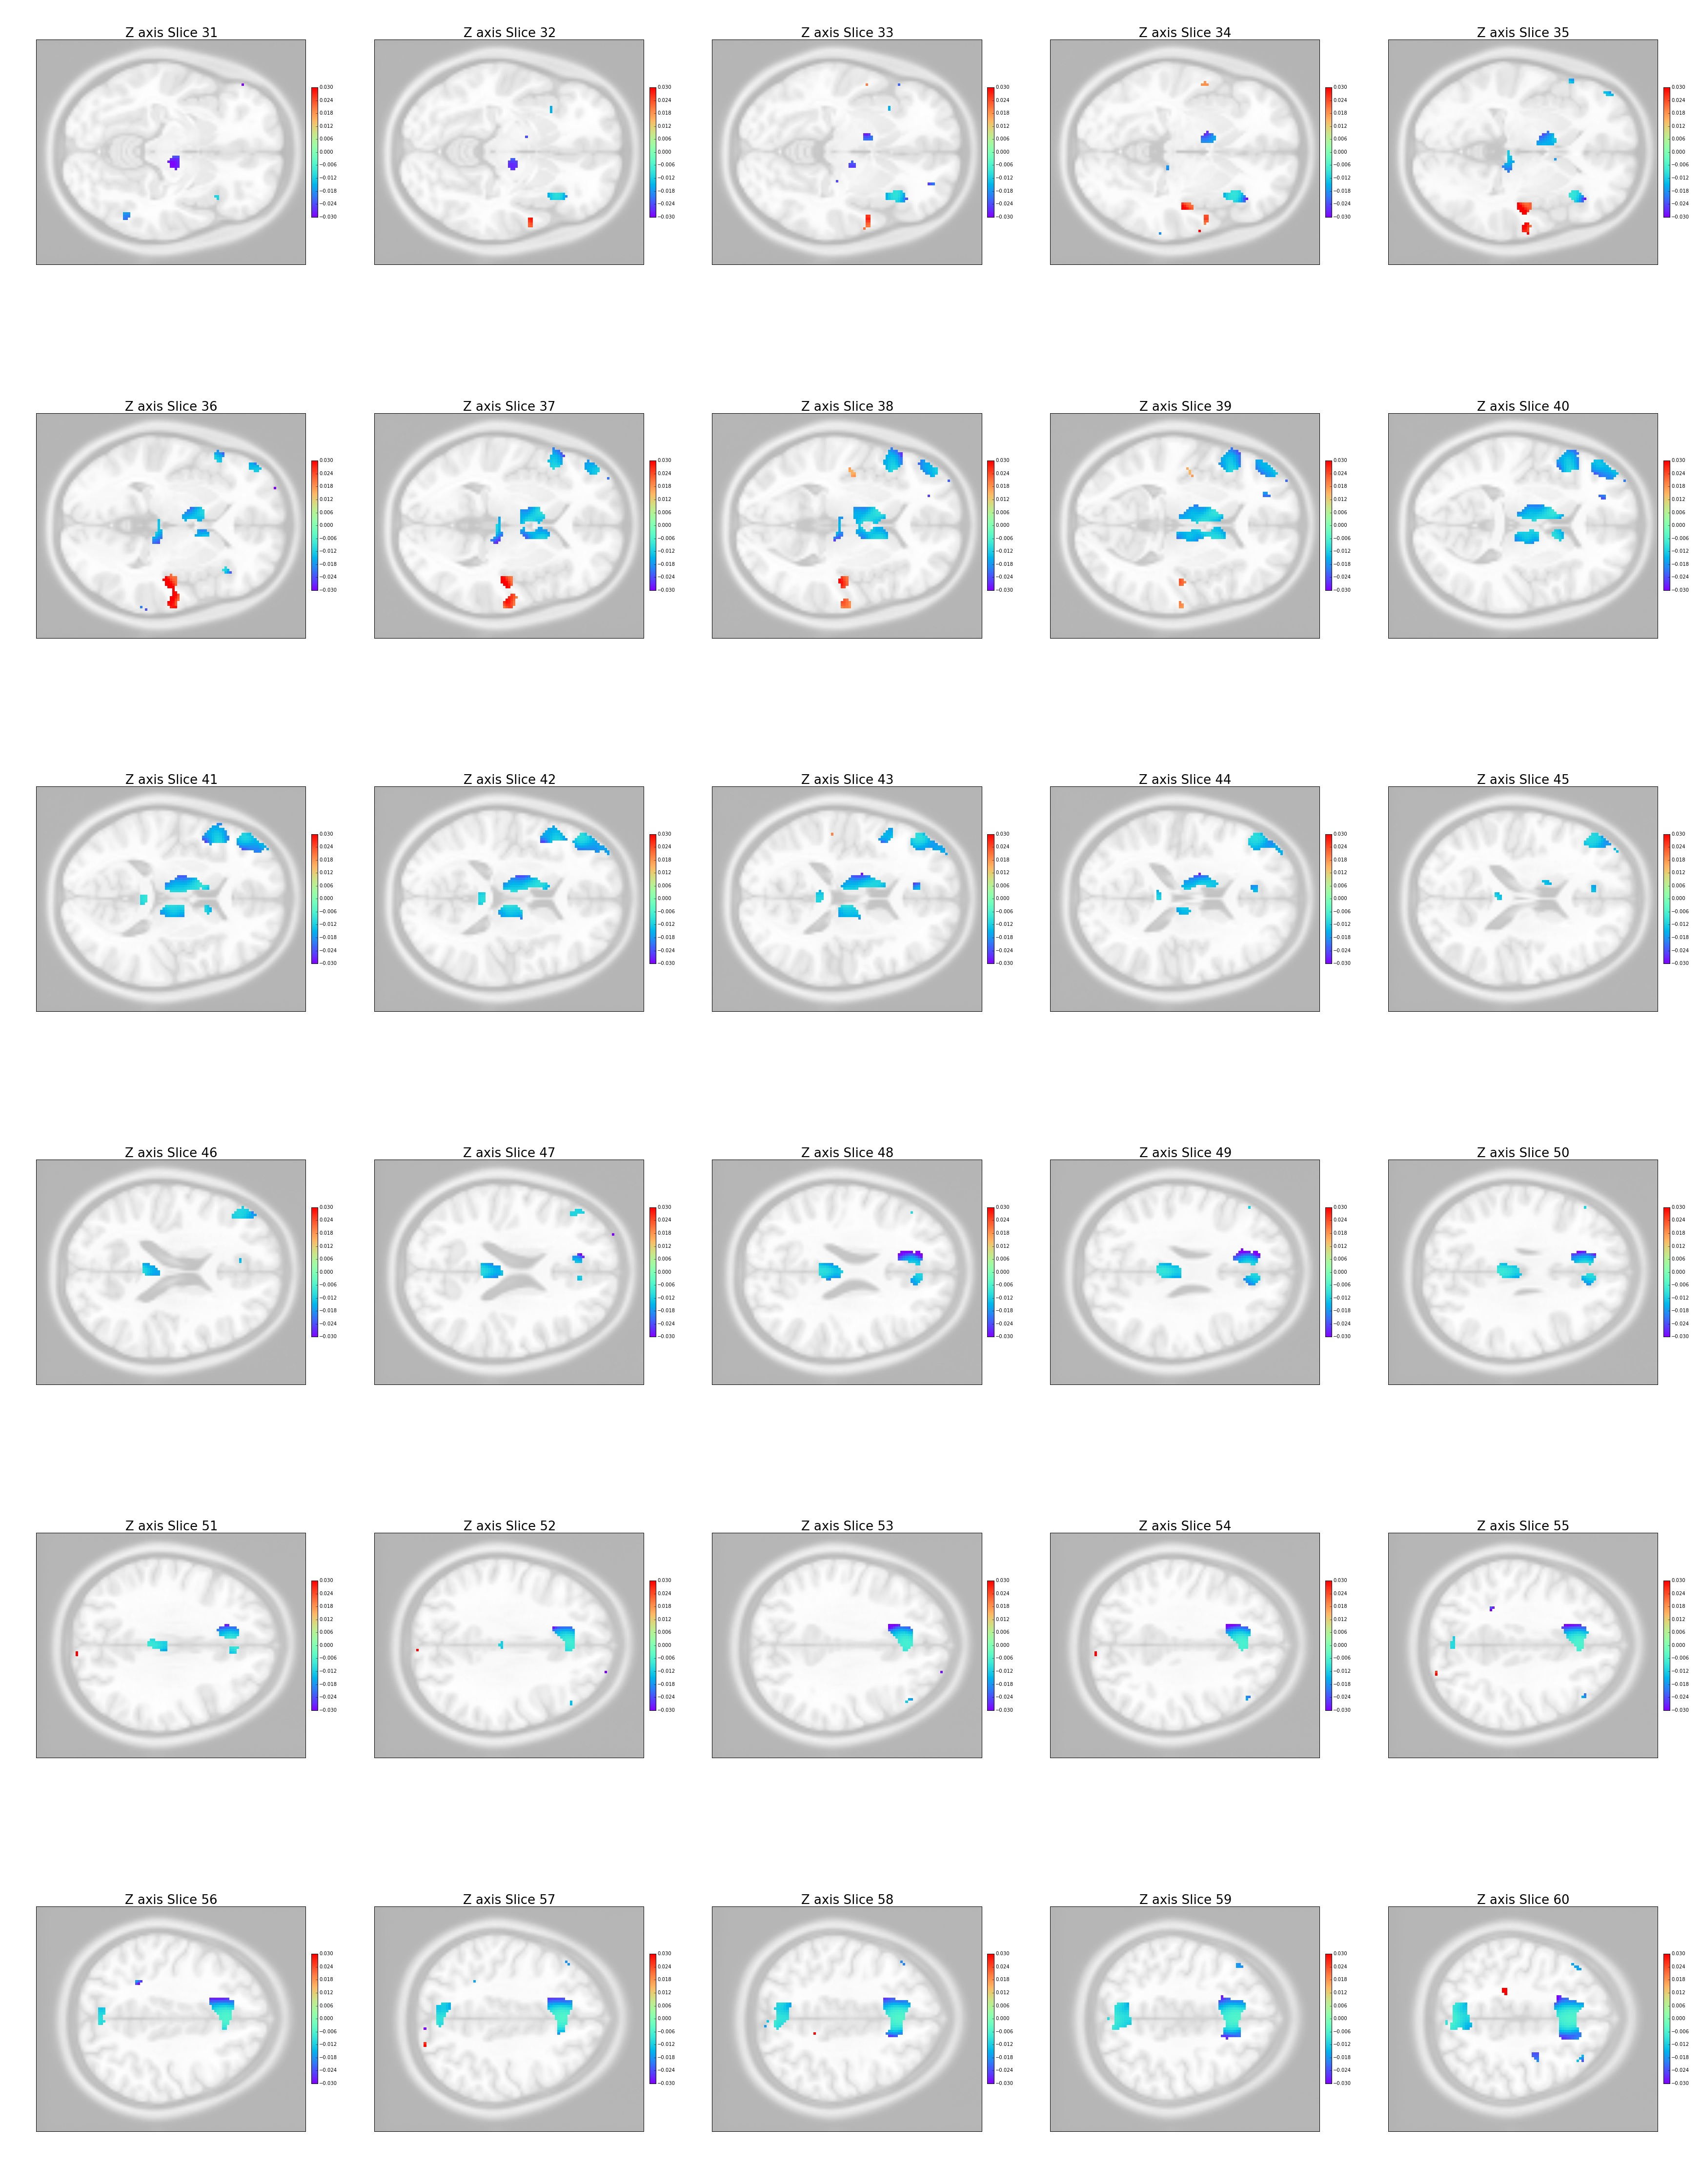
\includegraphics[scale=0.1]{figures/Regression3/sig_cor_z_loss.png}
    \caption{Our results: heat map of regions with significant correlation}
\end{figure}

\begin{figure}[H]
    \centering
        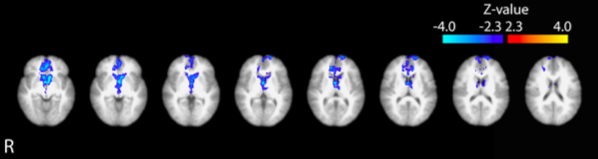
\includegraphics[scale=0.5]{figures/Regression3/Orig_sig_cor_z_loss.png}
    \caption{Original paper: Heat map of regions with significant correlation}
\end{figure}

\newpage

\emph{Figure S2} Regions with significant correlation between the parametric 
response to potential gains and behavioral loss aversion (ln($\lambda$)) across 
participants (Significant level = 0.001).  No regions showed significant 
negative correlation.

\begin{figure}[H]\label{sig_cor_z_gain}
    \centering
        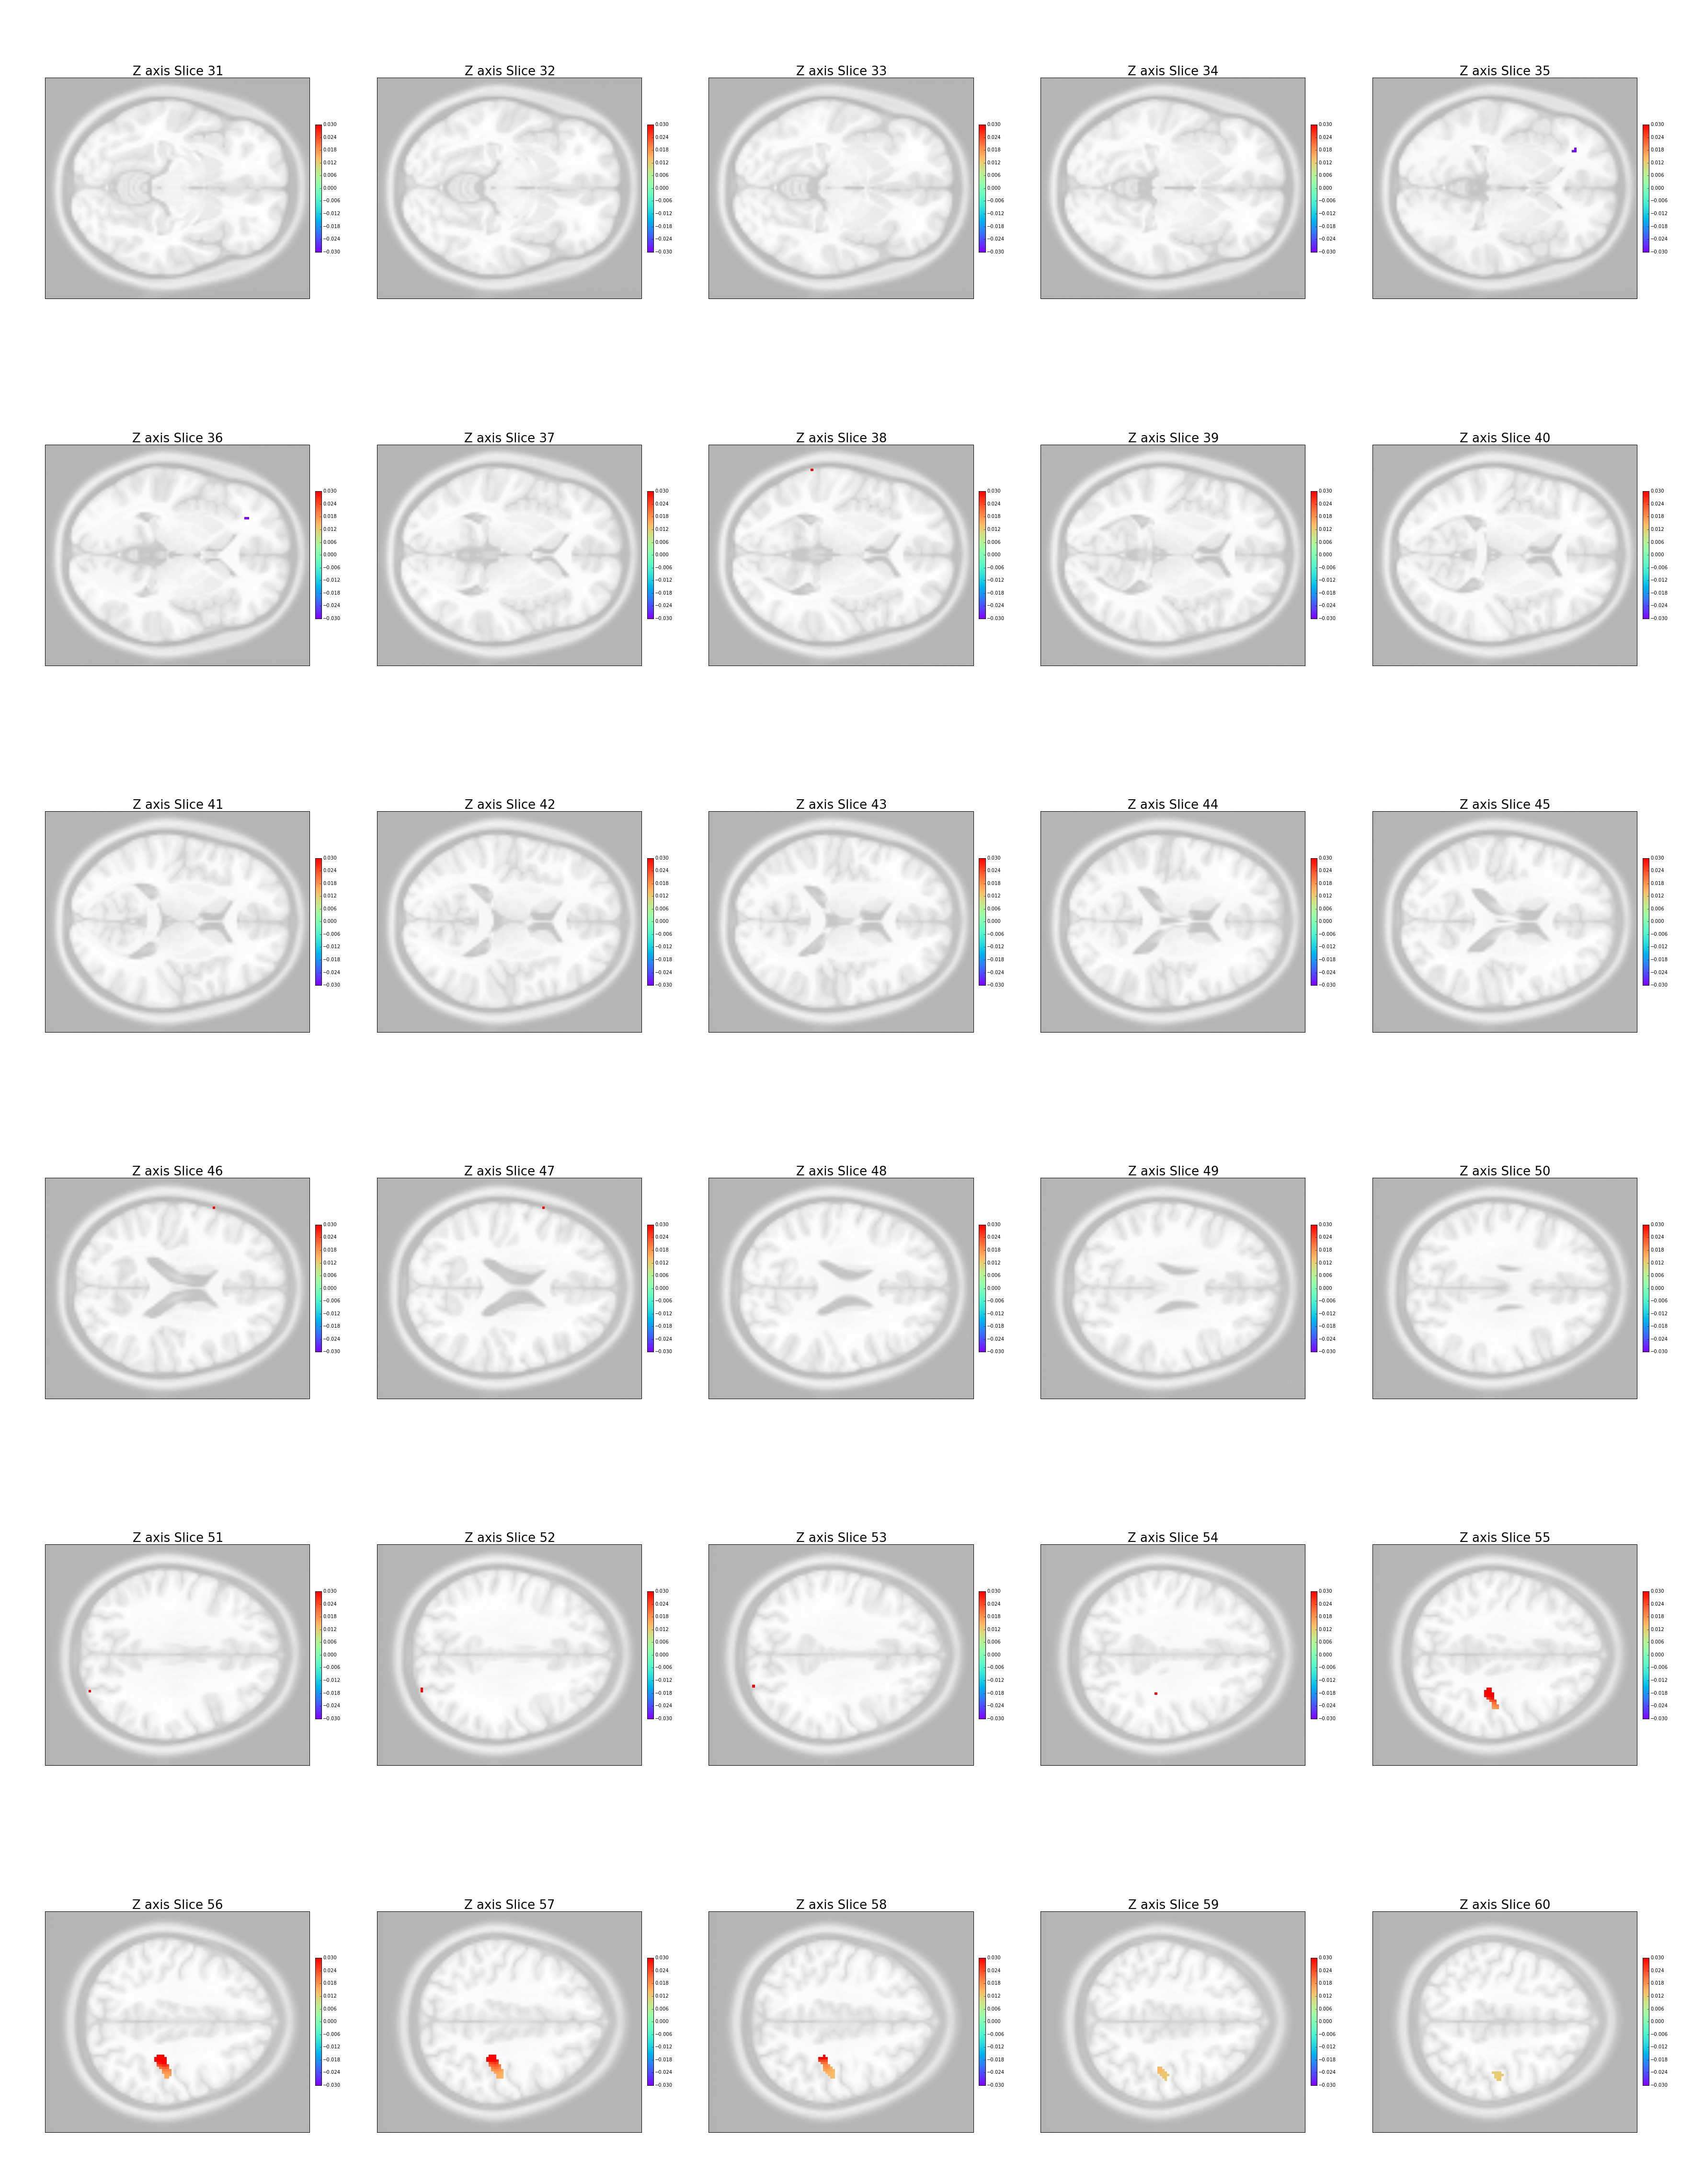
\includegraphics[scale=0.105]{figures/Regression3/sig_cor_z_gain.png}
    \caption{Our results: heatmap of regions with significant correlation}
\end{figure}

\begin{figure}[H]
    \centering
        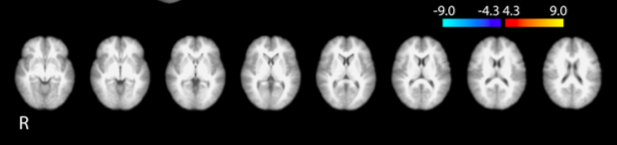
\includegraphics[scale=0.5]{figures/Regression3/Orig_sig_cor_z_gain.png}
    \caption{Original paper: Heatmap of regions with significant correlation}
\end{figure}

\newpage

\emph{Figure S3} Regions showing significant correlation between behavioral 
loss aversion ln($\lambda$) and neural loss aversion (difference between the 
absolute slopes of neural loss and gain responses) (Significant level = 0.001). 
There are both significant positive correlation and significant negative 
correlation. This result is different from the paper, in which no regions 
showed significant negative correlation.

\begin{figure}[H]
\centering
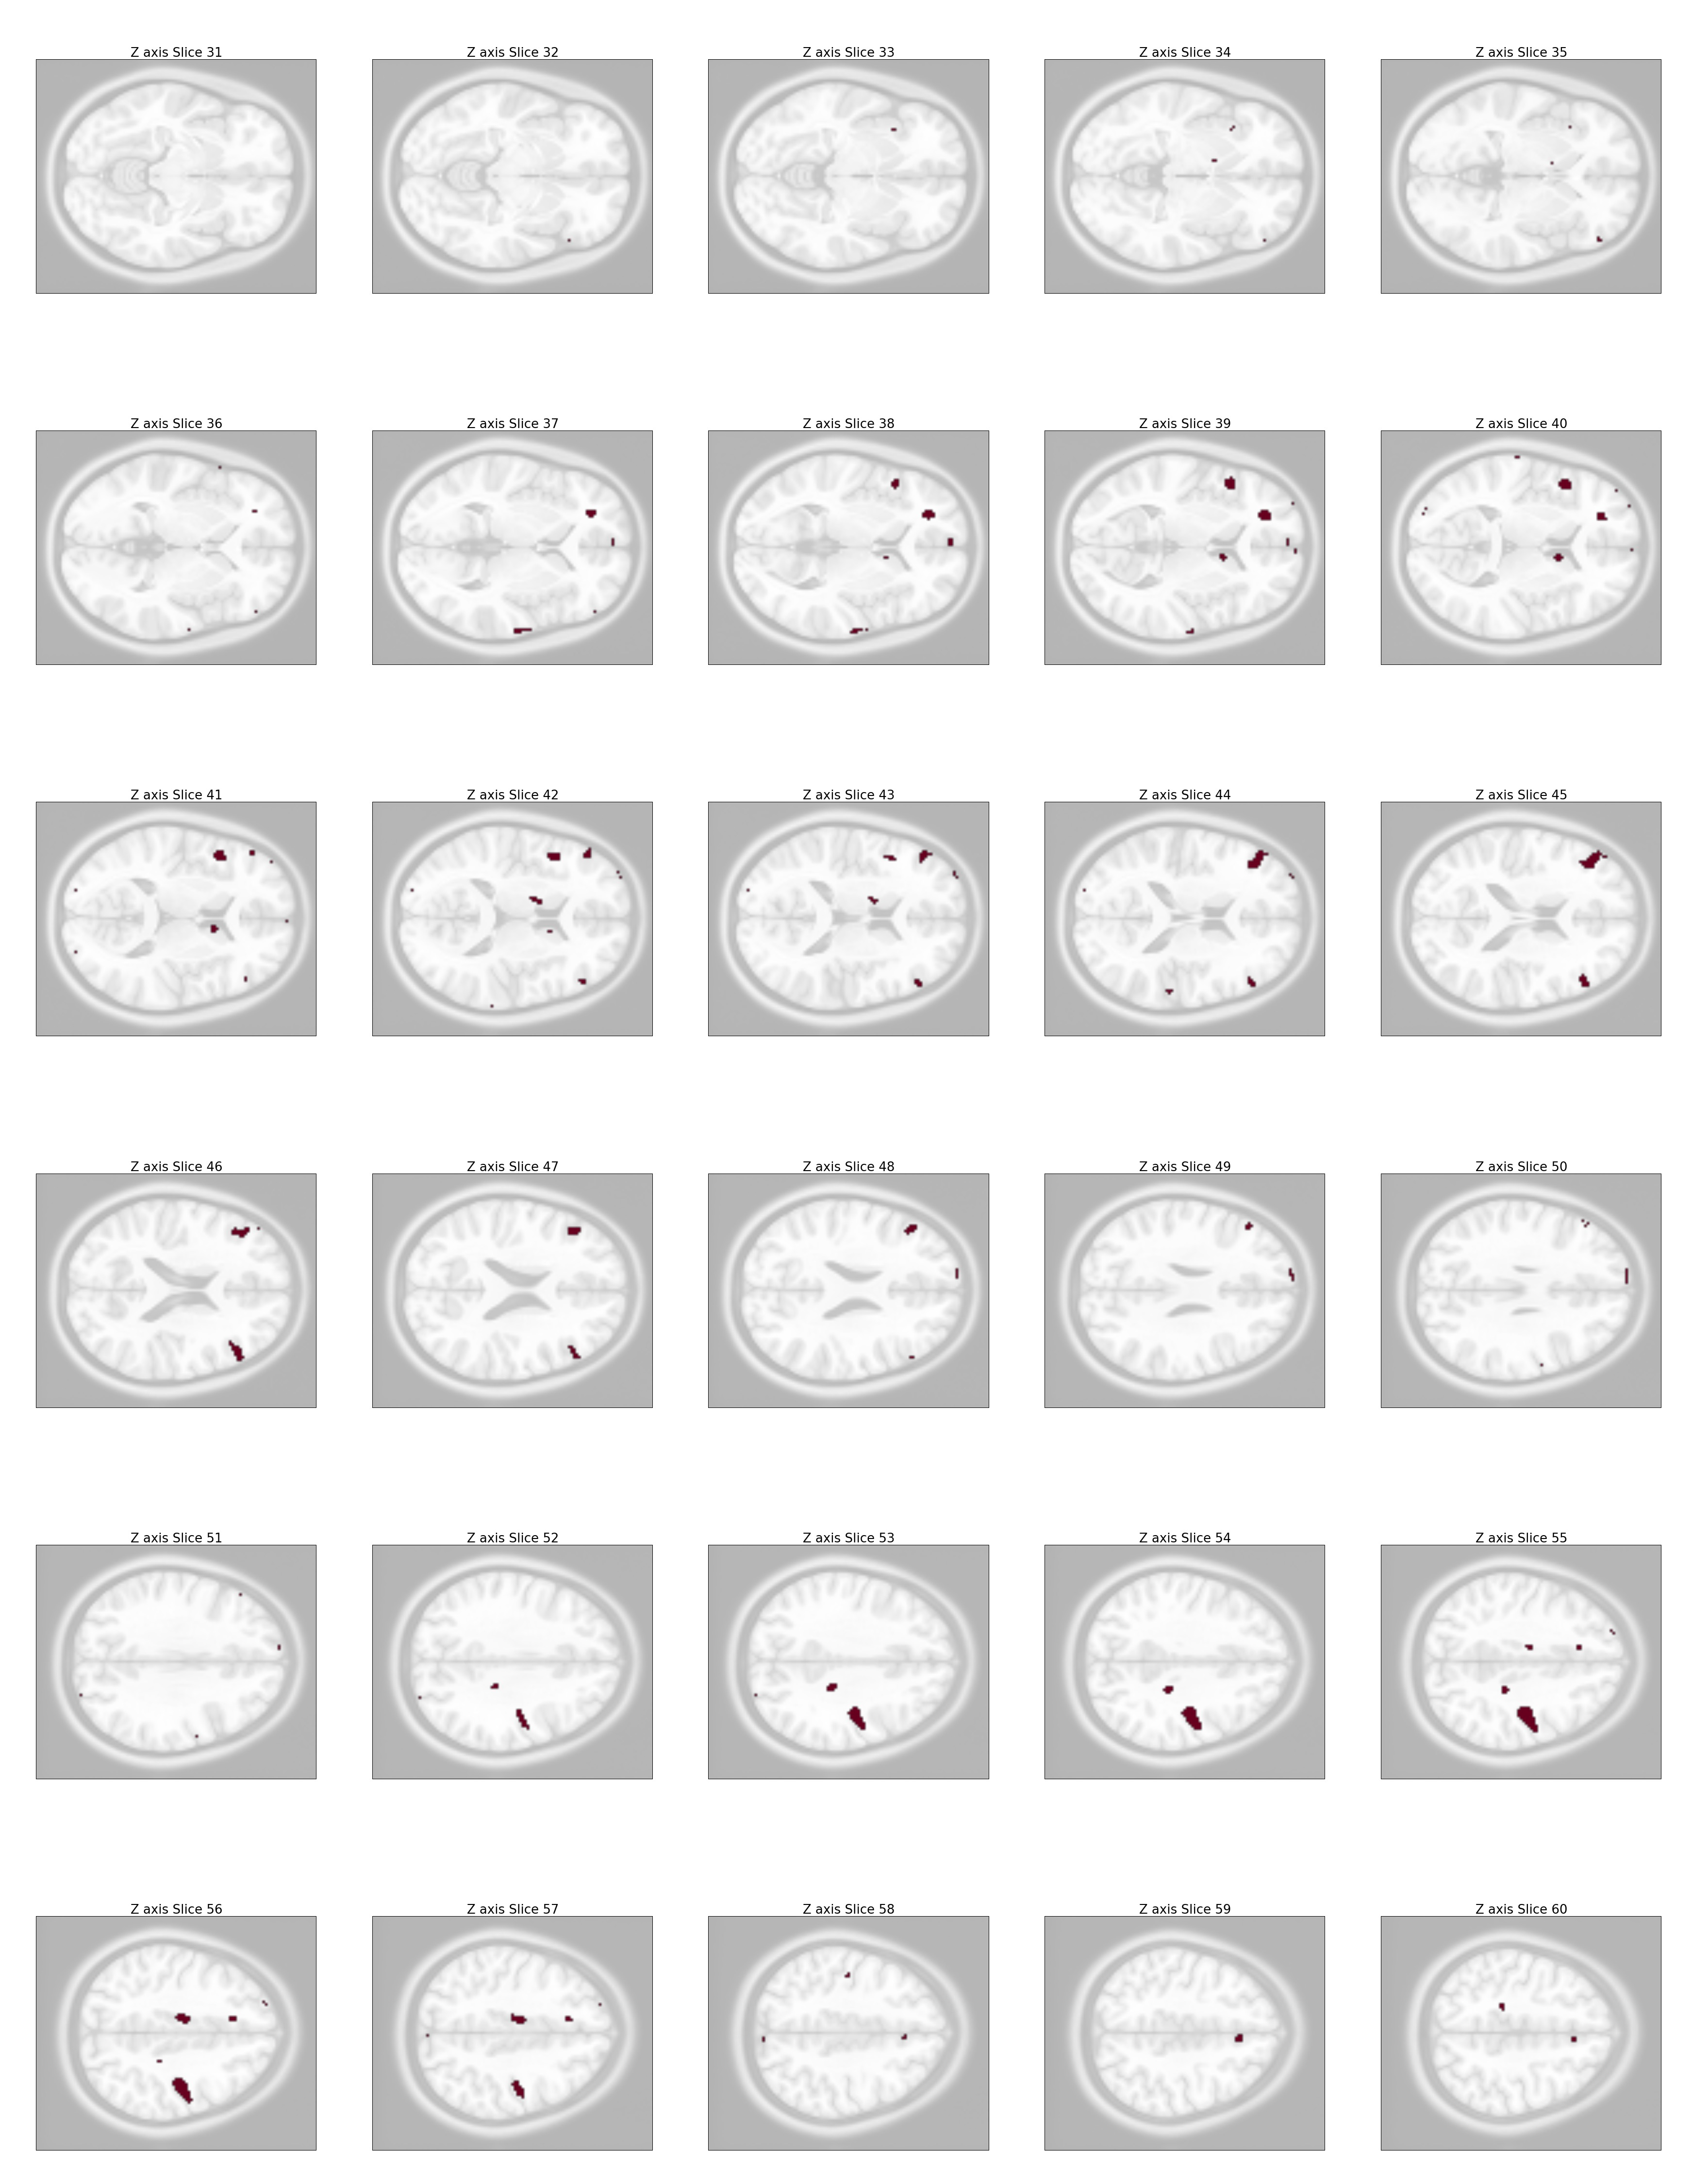
\includegraphics[scale=0.105]{figures/Regression3/sig_cor_z_neural_aversion.png}
\caption{Our results: heatmap of regions with significant correlation}
\end{figure}

\begin{figure}[H]
\centering
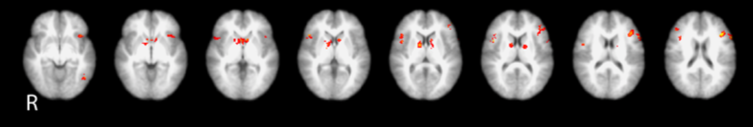
\includegraphics[scale=0.5]{figures/Regression3/Orig_sig_cor_z_neural_aversion.png}
\caption{Original paper: Heatmap of regions with significant correlation}
\end{figure}

\newpage

%\begin{figure}[H]
%    \centering
%        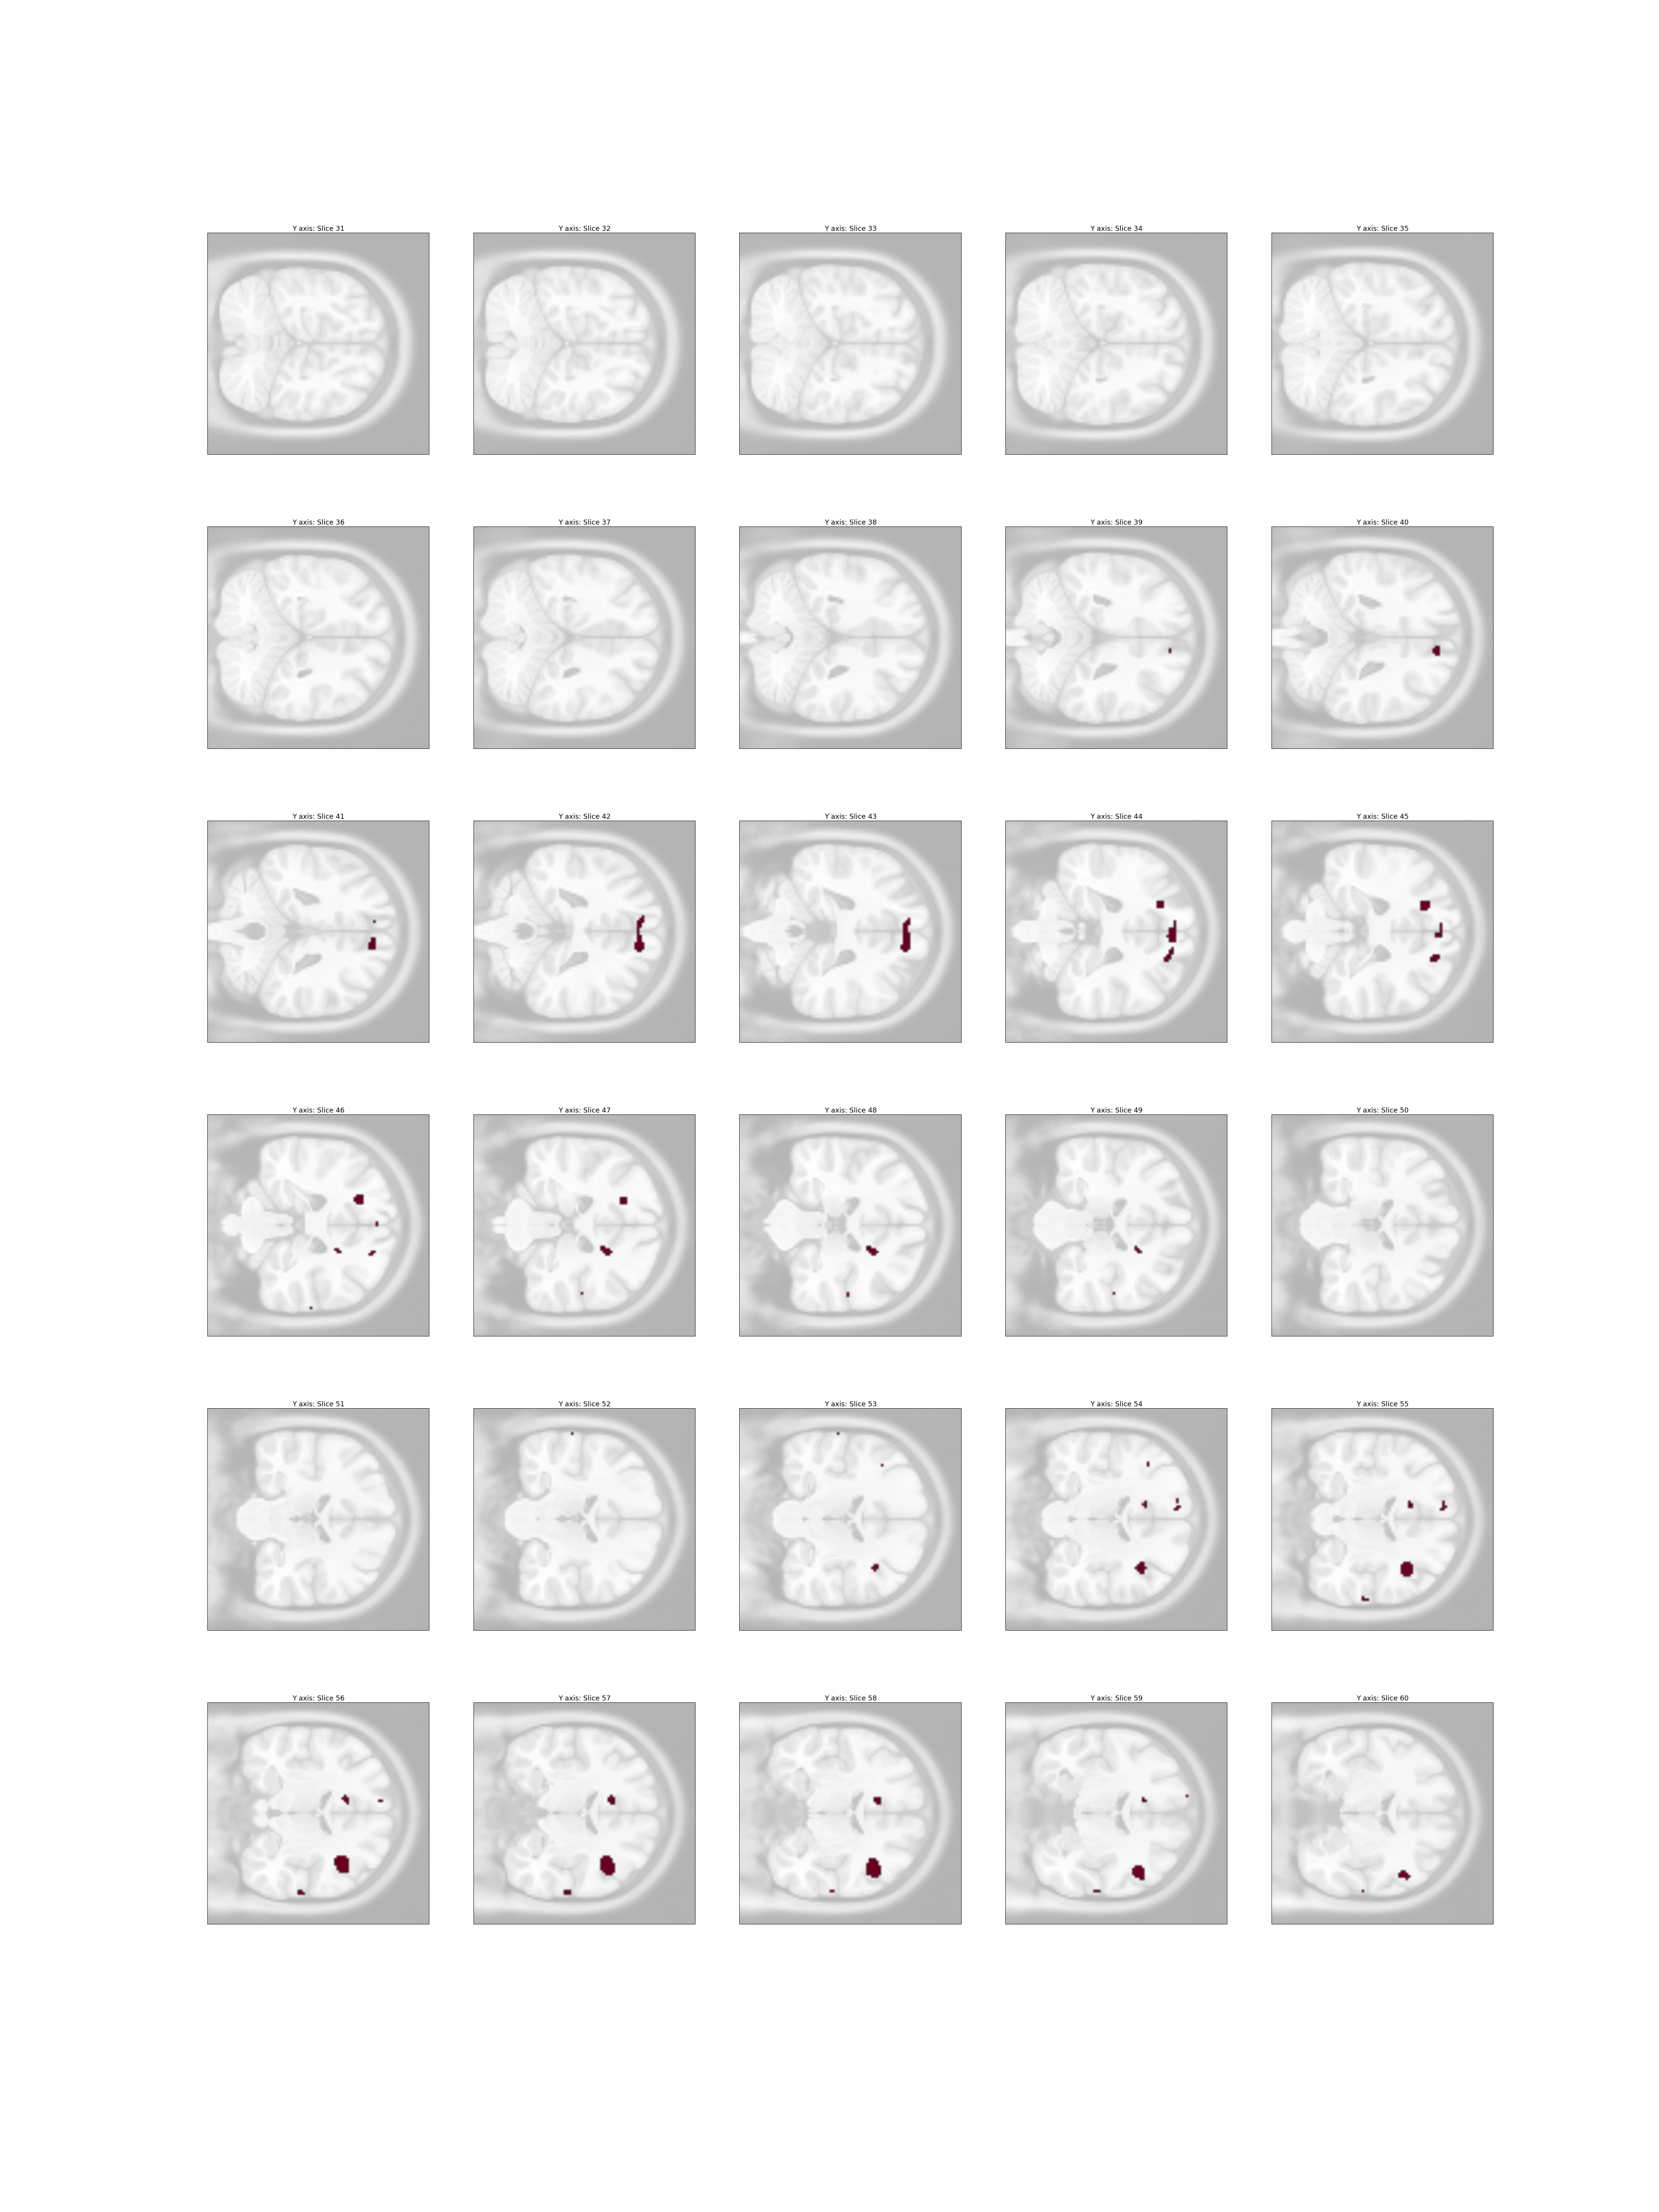
\includegraphics[scale=0.1]{figures/Regression3/sig_cor_y_neural_aversion.png}
%    \caption{Our results: heatmap of regions with significant correlation}
%\end{figure}

\section{Discussion}

\subsection{Issues with analyses and potential solutions}

\subsubsection{Selecting specific regions to further explore 
correlation between neural and behavioral activity}

\indent Since we have no knowledge on the sections of brain that might 
experience large difference in activation, it is hard for us to identify the 
specific regions in terms of anatomy to explore the correspondence between 
neural and behavioral loss aversion.

There are two potential ways to deal with this issue. The first one is a 
top-down approach to isolate potential regions of analysis. This method 
requires us to read more paper and related articles to better our anatomical 
understanding of the specific brain regions that are more likely to react in our 
given scenario -- loss aversion faced with potential gain and loss combinations.

Another way is a bottom-up approach. In this method, we can fit a regression for 
every part of the brain and look for the areas with higher correspondence 
(higher slope). Then, we select and graph a few areas with the most significant 
positive or negative correlation between the parametric response to potential 
losses and behavioral loss aversion (ln(λ)) across participants by knowing the 
standard template of neural response. This second method is what we have 
attempted to complete in our paper, conducting whole brain analysis using 
standardized filtered data (provided by Matthew Brett) and producing 
significant results to compare with those of Tom et al. Please see 
\textit{Methods} and \textit{Results} for further discussion of analysis 
procedures and results. 

\subsubsection{Run Time Issues}

One of the main issues is the run time of our analysis. More specifically, 
the scripts for running the mixed effects model is very time-exhaustive. On
our laptop, that script alone took over a day (Boying can confirm). Perhaps
this is due to the lower processing speeds on our laptops compared with the
standard desktop/research computing hardware used in standard fMRI research
settings. Additionally, by using the ds005 dataet with the standard mni 
template, the regression scripts takes more than 4 hours as well. This is due
to the significantly larger size of the filtered data (almost 15 GB). 
Nonetheless, we managed to complete our analysis and generated the figures 
shown in this paper in a reproducible pipeline. We also note that hardware 
improvements is not the only way to address run time issues. In terms of 
software, code optimization may be another way to decrease the run time. 
Specifically, we can explore a better balance between performance and clarity
with more experience in scientific computing and practice with code 
optimization.

\subsection{Further Research}

\par Looking at our data of subjects, it may be of interest to consider a 
demographic grouping by gender because our dataet contains the demographics of 
our 16 subjects, with the extra information of gender and age. A question to 
potentially address: Is there a significant difference to loss aversion across
genders?

\par Additionally, it is interesting to see that the behavioral data contains a 
column for the response time of each gambling task. To further explore how 
decision are made in gambling task, we can use the response time as one of the 
logistic regressors. Through step-wise or criterion based model selection 
methods (eg. AIC and backward elimination), we can attempt to find the best 
regressors that influence loss aversion to most.

% Subsection of Discussion
\subsection{Discussion of Challenges}

\par \indent One of the major challenges is trying to make this project as 
reproducible as possible while following guidelines on documentation, testing 
functions, and attempting to produce the results of the paper using our limited
understanding of fMRI data. Travis CI bugs with various versions of python, 
coverage failures, and errors with directory/path locations often hinder the 
process of smooth work-flows. Collaboration between five group members is no 
doubt difficult as we found it hard to come up with an attainable final goal 
that is still rewarding. 
\par Technically, most of us are new to python programming and research using 
git workflows, thus we have only a preliminary understanding of the various 
python resources available for our use. Additionally, lack of statistical 
understanding of some aspects of the paper has urged us to do independent 
research. Yet the disconnect between theory and implementation has been a major 
obstacle because as we try to put our knowledge into practice, we realize that
many pre-packaged software used in the original paper are unavailable to us. 
In addressing this, we have made our best attempt at creating a fMRI analysis 
pipeline. 
\par Some problems can be solved or alleviated by defining checkpoints and 
makingthe effort to re-read the paper and ask questions. Further, as we 
familiarize ourselves more and more  with various python modules and toolkits, 
results can be easier to attain and interpret. Nonetheless, we believe we have 
made significant gain in our understanding of not only fMRI research, but more 
importantly, the process of creating collaborative and reproducible research and
navigating the rough learning road of scientific programming. 


\bibliography{project}

\end{document}
